% TWS-taVNS evidence review and parameter audit.
% Build: latexmk -pdf tws-tavns-evidence.tex   (or `make paper` from the repository root)
\documentclass[10pt,a4paper]{article}

\usepackage[utf8]{inputenc}
\usepackage[T1]{fontenc}
\usepackage{lmodern}
\usepackage[margin=2.2cm]{geometry}
\usepackage{microtype}
\usepackage{amsmath}
\usepackage{booktabs}
\usepackage{longtable}
\usepackage{tabularx}
\usepackage{array}
\usepackage{enumitem}
\usepackage[table]{xcolor}
\usepackage{tikz}
\usetikzlibrary{arrows.meta,positioning,shapes.geometric}
\usepackage[style=authoryear,backend=biber,maxcitenames=2,mincitenames=1,maxbibnames=6,minbibnames=3,
            uniquelist=false,uniquename=false,giveninits=true,doi=true,url=true,isbn=false,eprint=false,
            dashed=false,useprefix=true]{biblatex}
\addbibresource{references.bib}
\usepackage{xurl}
\usepackage[hidelinks]{hyperref}
\pdfstringdefDisableCommands{\def\,{ }\def\textmu{u}}

\setlist{itemsep=1pt,topsep=3pt}
\renewcommand{\arraystretch}{1.15}
\newcommand{\us}{\texorpdfstring{\,\textmu s}{ us}}
\newcommand{\becomes}{\texorpdfstring{$\rightarrow$}{to}}
\newcommand{\code}[1]{\texttt{\small #1}}
\newcommand{\lvl}[1]{\textsf{\small #1}}
\newcolumntype{L}[1]{>{\raggedright\arraybackslash}p{#1}}
\newcolumntype{Y}{>{\raggedright\arraybackslash}X}

\title{TWS-taVNS: evidence review and parameter audit\\[2pt]
\large A closed-loop auricular vagus nerve stimulation earbud, checked value by value against the literature}
\author{TWS-taVNS project}
\date{22 November 2026}

\begin{document}
\maketitle

\begin{abstract}
\noindent TWS-taVNS is a software demonstration of an earbud that records ear-EEG, in-ear photoplethysmography (PPG) and
motion, detects seizures, and responds with transcutaneous auricular vagus nerve stimulation (taVNS) of the left cymba
conchae, behind a safety layer that can always stop it. This document audits every numeric parameter in the code
against primary sources. We checked 53 sources: every DOI was resolved through its registry, and every number quoted
taken from a source was read in its abstract or full text during this review. Of 35 parameters, 13 are supported by
direct evidence and kept, 8 were changed to match the evidence, 2 were added (a current-density limit and the electrode
area it needs), and 12 are labelled as design choices with no direct evidence. The review found one safety defect: the PPG heart-rate estimator could not see rates below
36\,bpm and reported the second harmonic instead, so a true 24--30\,bpm bradycardia read as 48--60\,bpm and did not lock
stimulation. That defect is fixed and covered by tests. All changes are listed in Section~\ref{sec:changes}.
\end{abstract}

\tableofcontents
\bigskip

%=====================================================================================================================
\section{Scope and method}\label{sec:method}

\paragraph{What was audited.} The Python package \code{tws/} (signal processing, detector, safety gate, state machine,
current limiter, simulator) and the values shown by the web and mobile apps. Comments in the code refer to an earlier
research write-up (``the doc'') for the scenarios and titration ranges. That write-up could not be opened from the
environment used for this review, so every value was re-derived from primary literature rather than copied from it.

\paragraph{How sources were verified.}
\begin{enumerate}
  \item Each DOI was resolved through \url{https://doi.org} and Crossref; the BibTeX in \code{references.bib} is the
        registry's own record, not retyped.
  \item Each number in this document was read in the source during the review. Table~\ref{tab:verification}
        (Appendix~\ref{app:log}) records where: \lvl{F} = full text (PubMed Central, Europe PMC, publisher PDF or
        official web page); \lvl{A} = abstract only; \lvl{S} = taken from a named secondary source because the primary
        full text was not accessible; \lvl{P} = public preview only; \lvl{M} = bibliographic metadata only (cited as a resource, no number taken).
  \item Parameters with no direct evidence are labelled \lvl{D} (design choice) with the reasoning, instead of being
        given a borrowed citation.
\end{enumerate}

\paragraph{What this document is not.} It does not validate the system on patient data; all results quoted for the
repository come from its simulator. It does not replace the text of IEC 60601-2-10, of which only the public preview
was read.

%=====================================================================================================================
\section{System overview}\label{sec:system}

The earbud sends a \code{SensorPacket} every 250\,ms: three EEG channels at 256\,Hz, PPG and a six-axis IMU at 48\,Hz,
per-channel electrode impedance, battery and fault flags. The core runs
\emph{link $\rightarrow$ signal $\rightarrow$ safety $\rightarrow$ stimulator}. The detector only proposes; the state
machine (Figure~\ref{fig:fsm}) decides, and the Locked and Safe-mode states override every request, scheduled ones
included. A software limiter checks each \code{StimCommand} before the stimulator sees it.

\begin{figure}[ht]
\centering
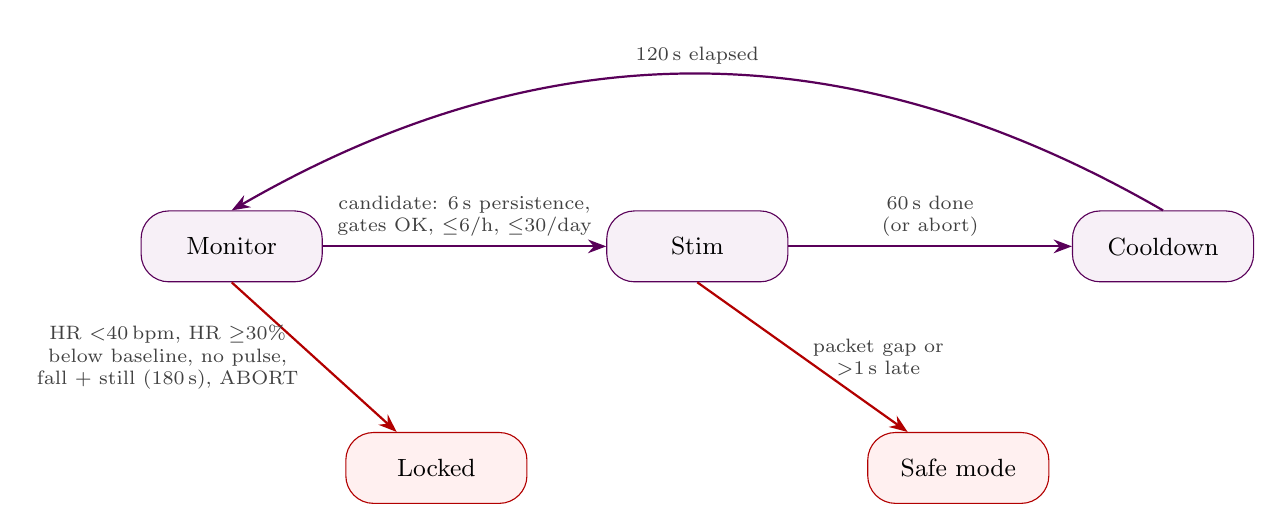
\begin{tikzpicture}[>=Stealth, node distance=2.4cm and 3.2cm,
  st/.style={draw=violet!70!black, fill=violet!6, rounded corners=10pt, minimum width=2.3cm, minimum height=0.9cm, font=\small},
  bad/.style={draw=red!70!black, fill=red!6, rounded corners=10pt, minimum width=2.3cm, minimum height=0.9cm, font=\small},
  lab/.style={font=\scriptsize, align=center, text=black!75}]
  \node[st] (mon) {Monitor};
  \node[st, right=3.6cm of mon] (stim) {Stim};
  \node[st, right=3.6cm of stim] (cd) {Cooldown};
  \node[bad, below=1.9cm of mon, xshift=2.6cm] (lock) {Locked};
  \node[bad, below=1.9cm of cd, xshift=-2.6cm] (safe) {Safe mode};
  \draw[->, thick, violet!70!black] (mon) -- node[lab, above] {candidate: 6\,s persistence,\\gates OK, $\le$6/h, $\le$30/day} (stim);
  \draw[->, thick, violet!70!black] (stim) -- node[lab, above] {60\,s done\\(or abort)} (cd);
  \draw[->, thick, violet!70!black] (cd.north) to[out=150, in=30] node[lab, above] {120\,s elapsed} (mon.north);
  \draw[->, thick, red!70!black] (mon.south) -- node[lab, left, xshift=-2pt] {HR $<$40\,bpm, HR $\ge$30\%\\below baseline, no pulse,\\fall + still (180\,s), ABORT} (lock);
  \draw[->, thick, red!70!black] (stim.south) -- node[lab, right] {packet gap or\\$>$1\,s late} (safe);
\end{tikzpicture}
\caption{State machine with the parameter values after this audit. Locked and Safe mode can be entered from every
state (only two arrows drawn); both abort a running stimulation, which still owes its cooldown.}
\label{fig:fsm}
\end{figure}

%=====================================================================================================================
\section{Stimulation site: left cymba conchae}\label{sec:site}

\textbf{Verdict: supported; kept (\code{SITE\_CYMBA\_LEFT}).}

\begin{itemize}
  \item \textcite{frangos2015} describe the cymba conchae as ``exclusively innervated by the ABVN'' and showed, in 12
        adults, that stimulating the left cymba conchae (continuous 0.25\,ms pulses at 25\,Hz) activated the ipsilateral
        nucleus tractus solitarii and the classical central vagal projections, compared with earlobe stimulation.
  \item \textcite{yakunina2017} compared four sites in 37 subjects (500\us{} pulses, 25\,Hz). Only cymba conchae
        stimulation produced significantly stronger activation than sham in both the nucleus tractus solitarii and the
        locus coeruleus; the ear canal gave the weakest activation.
  \item The anatomical basis is thinner than often stated. The most cited cadaver study \parencite{peuker2002} dissected
        14 ears of 7 cadavers, and \textcite{butt2020} document contradictions between its table and its text (for the
        tragus, antihelix and concha). Butt et al.\ conclude it is ``reasonable to surmise'' that the concha and inner
        tragus are suitable sites.
  \item Laterality: \textcite{kim2022} report that 71.3\% of the taVNS studies they reviewed used the left side, and that
        the few right or bilateral studies carried no additional risk in their analysis. The left side is the
        convention, not a proven requirement.
  \item The device with an epilepsy indication uses the same site: NEMOS stimulates the left cymba conchae and holds a
        CE mark for drug-resistant epilepsy \parencite{yap2020}.
\end{itemize}

%=====================================================================================================================
\section{Stimulation dose}\label{sec:dose}

\subsection{Frequency and pulse width (25\,Hz, 250\us)}\label{sec:freq}
\textbf{Verdict: supported; kept.} 25\,Hz with 0.25\,ms pulses at the left cymba conchae is the protocol of
\textcite{frangos2015}, and of the cMPsE02 epilepsy trial \parencite{bauer2016}, whose NEMOS settings
\textcite[Table 2]{yap2020} tabulate as 0.25\,ms, 25\,Hz, 30\,s on / 30\,s off for 4\,h a day. NEMOS delivers continuous
biphasic square pulses of 0.25\,ms at 25\,Hz \parencite[Gancheva et al.\ row]{farmer2020}. Of 177 taVNS studies, 145
used 20--30\,Hz (24 used 1--20\,Hz), and 80 used pulse widths of 0--250\us{} (55 used 300\us{} or more)
\parencite[Table 1, summed over its three columns]{kim2022}.

The limiter range of 1--30\,Hz spans the 1\,Hz active control of cMPsE02 \parencite{bauer2016} and the top of the
20--30\,Hz band. The 500\us{} pulse-width cap is the widest pulse tested by \textcite{badran2018}, who found 60\,s trains
safe and tolerable at 200\% of perceptual threshold, and by \textcite{yakunina2017}.

\subsection{Amplitude (1.0\,mA default, 5\,mA cap)}\label{sec:amp}
\textbf{Verdict: default supported as a titration start; cap is a design value inside the reported range.}
taVNS amplitude is titrated per person to a perceptible, non-painful level. Reported means are:
\begin{itemize}
  \item cMPsE02: $0.50\pm0.47$\,mA in the 25\,Hz arm and $1.02\pm0.83$\,mA in the 1\,Hz arm \parencite{bauer2016}.
  \item Frangos et al.: 0.3--0.8\,mA \parencite[Table 2]{yap2020}; Gancheva et al.\ (NEMOS): 0.6--1.4\,mA
        \parencite{farmer2020}.
  \item Tragus perceptual thresholds fall with pulse width: $4.64\pm1.28$\,mA at 100\us, $2.66\pm0.80$\,mA at 200\us{}
        and $1.5\pm0.47$\,mA at 500\us; delivered currents at 200\% of threshold were $5.32\pm1.60$\,mA at 200\us{} and
        $3.0\pm0.93$\,mA at 500\us{} \parencite{badran2018}.
\end{itemize}
The 1.0\,mA default sits inside the cymba conchae range above. The 5\,mA cap covers every cymba conchae mean listed
and the 500\us{} tragus condition (3.0\,mA), but not the shorter-pulse tragus conditions (5.32\,mA at 200\us,
9.28\,mA at 100\us), which the system does not use. Per-person titration is outside the code.

\subsection{On-time of a responsive stimulation: 30\,s \becomes{} 60\,s}\label{sec:ontime}
\textbf{Verdict: changed to 60\,s.} No taVNS trial has tested seizure-triggered stimulation, so the closest evidence is
implanted closed-loop VNS. In the E-37 trial of AspireSR \parencite{fisher2016}, AutoStim (triggered by ictal
tachycardia) used 0.75--1.5\,mA, 250--500\us{} and an \emph{on time of 60\,s}; Magnet Mode also used 60\,s. Of 31
seizures treated by AutoStim, 19 (61.3\%) ended during stimulation, with a median of 35\,s from stimulation onset to
seizure end. In an earlier multicentre study of the same cardiac-based detection \parencite{boon2015}, seizure activity stopped
during stimulation in 10 of the 17 seizures where triggered VNS overlapped ongoing seizure activity.

A 30\,s train would end before the median E-37 seizure did. 60\,s matches the AutoStim on-time and is the train length
\textcite{badran2018} found safe for taVNS. \code{FsmConfig.responsive\_s} and the limiter cap were both raised to 60\,s.

\subsection{Duty cycle, cooldown and rate caps}\label{sec:duty}
Intermittent stimulation widens the margin against stimulation-induced nerve injury, which in animal models came from
continuous high-frequency stimulation \parencite{agnew1990}. The settings give:
\begin{itemize}
  \item \textbf{Cooldown 120\,s} (\lvl{D}, kept): after a 60\,s train, at most 33\% on-time locally. NEMOS ran a
        50\% cycle (30\,s on / 30\,s off) for 4\,h a day \parencite[Table 2]{yap2020}, so this is more conservative.
  \item \textbf{6 per hour} (kept, now evidence-anchored): $6\times60$\,s is 10\% hourly duty, the duty cycle of VNS
        Normal Mode, about 11 stimulations per hour \parencite{fisher2016}. In E-37 the mean duty cycle rose from 11\% to 16\% at six
        months with AutoStim added.
  \item \textbf{30 per day} (\lvl{D}, kept): at most 30\,min of responsive stimulation a day, well below the 4--5\,h a
        day of NEMOS use \parencite{yap2020}. With reported false-detection rates of 0.49--2.8 per 24\,h for
        behind-the-ear detectors \parencite{vandecasteele2020}, the cap only binds in clusters.
  \item \textbf{Scheduled session 1800\,s} (kept): 30\,min sits inside the published range of 3\,$\times$\,20\,min a
        day \parencite{aihua2014}, 3\,$\times$\,30\,min a day \parencite{he2013} and 3\,$\times$\,1\,h a day
        \parencite{stefan2012}, all as tabulated by \textcite{yap2020}. Scheduled sessions count towards the same
        caps.
\end{itemize}

\subsection{Electrical safety and the new current-density check}\label{sec:electrical}
\textbf{Verdict: limiter extended.} Stimulator safety depends on charge per phase and on current density at the skin,
not on amplitude and pulse width separately. For the symmetric biphasic pulses NEMOS uses \parencite{farmer2020},
amplitude $I$, phase width $t_p$ and frequency $f$ give
\begin{equation}
Q_{\text{phase}} = I\,t_p, \qquad I_{\text{rms}} = I\sqrt{2\,t_p\,f}, \qquad J_{\text{rms}} = I_{\text{rms}}/A .
\end{equation}
For the closest US device class with a cranial transcutaneous target, stimulators to treat headache, 21 CFR 882.5891
requires the maximum phase charge, net charge per pulse, maximum current density (mA/cm$^2$ r.m.s.) and average power
density to be characterised \parencite{cfr8825891}. A 2024 FDA-published
510(k) summary cites ``safety limits of 2\,mA/cm$^2$ and 0.25\,W/cm$^2$'' for its IEC 60601-2-10 risk analysis
\parencite{fdak241678}; the standard itself covers nerve and muscle stimulators \parencite{iec60601210}. Charge-balanced
waveforms follow from the electrochemistry of charge injection reviewed by \textcite{merrill2005}.

\begin{table}[ht]
\centering\small
\begin{tabularx}{\textwidth}{L{3.6cm}YYYYY}
\toprule
Setting & $Q_{\text{phase}}$ & $I_{\text{rms}}$ & $J_{\text{rms}}$ at 0.5\,cm$^2$ & Minimum area for 2\,mA/cm$^2$ & Power density at 500\,$\Omega$ \\
\midrule
Default: 1.0\,mA, 250\us, 25\,Hz & 0.25\,\textmu C & 0.112\,mA & 0.22\,mA/cm$^2$ & 0.056\,cm$^2$ & 0.013\,mW/cm$^2$ \\
Limiter maximum: 5\,mA, 500\us, 30\,Hz & 2.5\,\textmu C & 0.866\,mA & 1.73\,mA/cm$^2$ & 0.433\,cm$^2$ & 0.75\,mW/cm$^2$ \\
\bottomrule
\end{tabularx}
\caption{Charge and density for symmetric biphasic pulses, from Eq.~(1). The 0.5\,cm$^2$ electrode area is a placeholder
until the earbud electrode is measured. Power density is far below the 0.25\,W/cm$^2$ benchmark in both cases.}
\label{tab:charge}
\end{table}

The limiter now rejects any command whose r.m.s.\ current density exceeds 2\,mA/cm$^2$ for the configured electrode area
(\code{Limits.electrode\_area\_cm2}). The stimulating electrode must have at least 0.433\,cm$^2$ of contact for the
widest settings to pass (Table~\ref{tab:charge}).

\subsection{Clinical evidence that taVNS reduces seizures}\label{sec:efficacy}
The evidence is for \emph{scheduled} (open-loop) taVNS. None of these trials tested stimulation triggered by a detected
seizure.

\begin{table}[ht]
\centering\small
\begin{tabularx}{\textwidth}{L{3.1cm}L{2.7cm}Y}
\toprule
Study & Design & Result (as reported) \\
\midrule
\textcite{stefan2012} & Pilot, $n=10$, 9 months & 3 dropped out; seizure frequency fell in 5 of the remaining 7 \\
\textcite{he2013} & Pilot, $n=14$ children, 24 weeks & Mean seizure reduction 54.21\% at weeks 17--24; responder rate 53.85\% \\
\textcite{rong2014} & RCT, $n=144$ (98 vs.\ 46) & After 8 weeks, mean seizure frequency fell 42.6\% vs.\ 11.5\% ($P<0.05$) \\
\textcite{aihua2014} & Controlled, $n=60$, 12 months & Monthly seizures 8.0 $\rightarrow$ 4.0 in the treatment group ($P=0.003$) \\
\textcite{bauer2016} (cMPsE02) & RCT, 25\,Hz $n=39$ vs.\ 1\,Hz $n=37$, 20 weeks & $-23.4\%$ vs.\ $-2.9\%$ per 28 days ($p=0.146$, not significant); 34.2\% in 25\,Hz completers ($p=0.034$) \\
\textcite{zhang2024} & Meta-analysis, 9 clinical studies, 788 patients & Response rate OR 2.94 (95\% CI 1.94--4.46) \\
\textcite{moro2025} & Meta-analysis, 4 RCTs, 368 patients & Monthly seizures MD $-3.01$ (95\% CI $-5.37$ to $-0.65$); responder OR 2.00 ($p=0.06$) \\
\bottomrule
\end{tabularx}
\caption{taVNS for epilepsy. Moro et al.\ note significant methodological concerns in some included trials.}
\label{tab:efficacy}
\end{table}

\subsection{Adverse events}\label{sec:ae}
\textcite{redgrave2018} pooled 51 studies with 1322 participants. The most common side effects were local skin
irritation (18.2\%), headache (3.6\%) and nasopharyngitis (1.7\%); 2.6\% dropped out for side effects; 3 of 30 serious
adverse events were judged possibly caused by tVNS. \textcite{kim2022} pooled 177 studies with 6322 participants and
found 12.84 adverse events per 100\,000 person-minutes-days of stimulation, no difference in risk between active and
control stimulation, and no causal link to severe events. cMPsE02 reported headache, ear pain, application-site
erythema, vertigo, fatigue and nausea \parencite{bauer2016}.

%=====================================================================================================================
\section{Seizure detection from ear-EEG}\label{sec:detect}

\subsection{Feasibility}
Simultaneous ear- and scalp-EEG in 15 patients with suspected temporal lobe epilepsy showed no difference in visual
seizure-detection sensitivity or specificity \parencite{zibrandtsen2017}. Ear-EEG performs like scalp EEG for
spectrum-based analysis of sources near the ear \parencite{mikkelsen2015}. Automated detectors on behind-the-ear channels
reached a median sensitivity of 94.5\% at 0.52 false detections per hour in 12 patients \parencite{gu2018}; 64.1\%
(patient-independent, 2.8 false positives per 24\,h) and 69.1\% (patient-specific, 0.49 per 24\,h) in 54 patients with
182 seizures \parencite{vandecasteele2020}; and 0.983 sensitivity for typical absences \parencite{swinnen2021}.

\subsection{Sampling and windows (256\,Hz, 2\,s windows, 1\,s stride)}
\textbf{Verdict: supported; kept.} The CHB-MIT database the repository targets for training was sampled at 256 samples
per second with 16-bit resolution. Its original 23 cases come from 22 paediatric subjects; with case chb24, added in
December 2010, the records hold 198 annotated seizures \parencite{chbmit2010,goldberger2000}. \textcite{shoeb2010} used 2\,s epochs, ``commonly used'' because EEG cannot be
segmented into shorter physiologically meaningful units.

\subsection{Frequency range: 12.5--25\,Hz \becomes{} eight bands over 0.5--25\,Hz}\label{sec:bands}
\textbf{Verdict: changed.} The original detector used one band, 12.5--25\,Hz. That misses common ictal rhythms:
\begin{itemize}
  \item hippocampal-onset seizures most specifically start with a regular 5--9\,Hz inferotemporal rhythm, and temporal
        neocortical seizures with irregular 2--5\,Hz activity \parencite{ebersole1996};
  \item typical absences are 3\,Hz spike-and-wave \parencite{swinnen2021};
  \item EMG has a broad spectrum with peaks at 20--30\,Hz (frontalis) and 40--80\,Hz (temporalis), and even weak
        contraction contaminates EEG above 12\,Hz \parencite{goncharova2003}. A beta-only detector is the band most
        exposed to chewing and jaw artefact.
\end{itemize}
\textcite{shoeb2010} span 0.5--25\,Hz with a filterbank of $M=8$ equal-bandwidth filters, ``since most seizure and
non-seizure EEG activity falls within this range''; on CHB-MIT their patient-specific detector found 96\% of 173 test
seizures with a mean latency of 4.6\,s and a median of 2 false detections per 24\,h. The detector now uses the same
eight 3.06\,Hz bands and scores the largest band power, over channels and bands, relative to that patient's calm
baseline for the band. The threshold (8, about 9\,dB) is \lvl{D} and must be fitted per patient. Line length
\parencite{esteller2001} and spectral entropy are computed but not yet used.

\subsection{Persistence: 4\,s \becomes{} 6\,s}
\textbf{Verdict: changed (\code{persist\_n} 3 $\rightarrow$ 5).} Shoeb and Guttag stack $W=3$ consecutive 2\,s epochs
(6\,s) because ``electroencephalographers require an EEG abnormality to persist and evolve for a minimum of 6--10
seconds'' \parencite{shoeb2010}. Five consecutive 2\,s windows at a 1\,s stride span 6\,s. In the simulator, detection
now comes 5\,s after seizure onset, close to the 4.6\,s mean latency above.

\subsection{Artefact rules}\label{sec:artefact}
The EMG index is the share of 1--100\,Hz power in 40--100\,Hz, the band where temporalis EMG peaks
\parencite{goncharova2003}; the band choice is supported. Both thresholds, peak-to-peak 300\,\textmu V and EMG share
0.25, are \lvl{D}. No source was found for ictal amplitude distributions in ear-EEG, so both must be calibrated on
recorded ictal ear-EEG. Tonic seizures carry heavy EMG and may be rejected as artefact. The IMU is deliberately not used
to reject artefact, because clonic movement is itself a seizure sign.

\subsection{Electrode impedance: \texorpdfstring{50\,k$\Omega$ \becomes{} 40\,k$\Omega$}{50 kOhm to 40 kOhm}}
\textbf{Verdict: changed.} With high input-impedance amplifiers, EEG amplitude did not change in any band as impedance
rose from under 10\,k$\Omega$ to 40\,k$\Omega$ \parencite{ferree2001}; nothing above 40\,k$\Omega$ was tested. The gate
now treats a channel above 40\,k$\Omega$ as unusable. Dry electrodes run at higher impedance and will need a value
measured on that hardware.

\subsection{Stimulation-artefact blanking (5\,ms)}
\lvl{D}. Samples within 5\,ms after each pulse are interpolated, which removes 12.5\% of samples at 25\,Hz. No published
blanking window for this electrode geometry was found; the value must be measured on the bench, including amplifier
recovery.

%=====================================================================================================================
\section{Safety gates}\label{sec:gates}

\subsection{Why heart rate gates stimulation}
\begin{itemize}
  \item Vagal stimulation can slow the heart. During implanted VNS lead testing (1.0\,mA, 20\,Hz, 500\us, about 17\,s)
        one patient developed bradycardia of about 30\,beats/min and then asystole; the manufacturer reported this in
        about 1 in 875 implants \parencite{asconape1999}.
  \item Seizures cause arrhythmias: \textcite{vanderlende2016} collected 103 cases of ictal asystole and 25 of ictal
        bradycardia, with a mean prevalence of ictal asystole of 0.318\% in people with refractory epilepsy undergoing
        video-EEG. In sleep-related hypermotor epilepsy, three of four analysed ictal bradycardias reached minimum rates
        of 4.5--9.3\,bpm \parencite{muccioli2024}.
  \item In MORTEMUS, sudden death after a generalised tonic-clonic seizure followed a pattern of rapid breathing
        (18--50 breaths/min) and then, within 3\,min, transient or terminal cardiorespiratory dysfunction
        \parencite{ryvlin2013}.
  \item taVNS itself moves heart rate very little: a mean of $-1.43$\,bpm across conditions, and at most $-3.13$\,bpm
        (500\us, 25\,Hz) \parencite{badran2018}. A gate tuned to large drops will not fire on the therapy's own effect.
  \item Ictal \emph{tachycardia} is the common case: it occurs in 82\% of patients \parencite{eggleston2014}.
\end{itemize}

\subsection{Heart rate from in-ear PPG: band 0.6--3.5\,Hz \becomes{} 0.4--3.5\,Hz plus harmonic check}\label{sec:ppg}
\textbf{Verdict: changed; this fixes a safety defect.} In-ear PPG pulse rate agreed with ECG within a mean absolute
percentage error of $\le$5\% but is sensitive to motion \parencite{passler2019}. The ear canal kept its PPG amplitude
during peripheral vasoconstriction, when finger sensors dropped by about half \parencite{budidha2014}. 48\,Hz satisfies
the $\ge$25\,Hz that \textcite{choi2017} found sufficient for pulse-rate variability.

The old estimator searched for the spectral peak in 0.6--3.5\,Hz (36--210\,bpm). Ictal bradycardia is defined from an
R--R interval of $\ge$2\,s, i.e.\ $\le$30\,bpm \parencite{muccioli2024}, and VNS-induced bradycardia was about 30\,bpm
\parencite{asconape1999}. Those rates were outside the search band. A real PPG has a strong second harmonic, so the
estimator reported the harmonic as a normal rate and the gate did not lock (Table~\ref{tab:ppgbug}).

\begin{table}[ht]
\centering\small
\begin{tabular}{lccccc}
\toprule
True heart rate (bpm) & 24 & 26 & 28 & 30 & 32 \\
\midrule
Before, 2nd harmonic 0.5$\times$: reading (lock?) & 47.8 (no) & 52.5 (no) & 56.2 (no) & 36.6 (yes) & 36.6 (yes) \\
Before, 2nd harmonic 1.0$\times$: reading (lock?) & 47.8 (no) & 52.5 (no) & 56.2 (no) & 60.0 (no) & 63.8 (no) \\
After, both cases: reading (lock?) & 24.4 (yes) & 26.2 (yes) & 28.1 (yes) & 30.0 (yes) & 31.9 (yes) \\
\bottomrule
\end{tabular}
\caption{Synthetic PPG (fundamental plus second harmonic, 12\,s at 48\,Hz) through \code{hr\_from\_ppg} and the safety
gate, before and after the fix. Readings of 36.6 were the band edge, not a measurement.}
\label{tab:ppgbug}
\end{table}

The band now starts at 0.4\,Hz (24\,bpm). If half the peak frequency, down to 0.25\,Hz, also holds at least a quarter of
the peak power, the lower frequency is taken as the pulse rate. The check errs towards the lower reading: a false low
reading locks, which is safe, while a harmonic read as normal is not. Respiration modulates the PPG baseline, amplitude
and frequency \parencite{charlton2018}, and post-convulsive breathing reached 18--50/min in MORTEMUS
\parencite{ryvlin2013}. Respiration can therefore still produce false low readings; these lock rather than unlock.
Regression tests cover 24--35\,bpm with harmonic ratios of 0.5--1.5 and 45--180\,bpm normal rates.

\subsection{Heart-rate thresholds}
\begin{itemize}
  \item \textbf{Absolute floor 40\,bpm} (kept). Sinus bradycardia is a rate below 50\,bpm, and the guideline's
        diagnostic pathway applies that cut-off ``while awake'' \parencite{acc2018gms,kusumoto2019}. 40\,bpm sits
        between that definition and the $\approx$30\,bpm of ictal and VNS-induced bradycardia above, and above the
        35\,bpm that \textcite{badran2018} monitored as an extreme decrease.
  \item \textbf{Relative drop 30\%} (\lvl{D}, kept). Definitions of ictal bradycardia range from a $\ge$10\% fall from
        baseline to an R--R interval of $\ge$2\,s \parencite{muccioli2024}; one of their cases fell 27\% (103 to
        75\,bpm). 30\% keeps false locks rare and stays far above the 1--3\,bpm effect of taVNS. Profound drops are
        caught by the absolute floor and by the no-pulse path.
  \item \textbf{Recovery within 10\%} and \textbf{30\,s minimum baseline} (\lvl{D}, kept).
  \item \textbf{Baseline window 300\,s} (kept): 5\,min is the conventional short-term heart-rate-variability recording
        \parencite{shaffer2017}. Separate sleep and awake baselines are kept because autonomic balance shifts towards
        parasympathetic dominance in NREM sleep and heart rate shows a circadian effect \parencite{trinder2001}.
\end{itemize}

\subsection{Fall then stillness: hold 60\,s \becomes{} 180\,s}\label{sec:fall}
\textbf{Verdict: hold changed; detection thresholds \lvl{D}.} An accelerometer in a behind-the-ear hearing-aid housing
detected falls with three thresholds: horizontal-plane acceleration $>2$\,g, velocity before impact $>0.7$\,m/s and
total acceleration $>6$\,g \parencite{lindemann2005}. Simple head- and waist-worn thresholds reached 97--98\%
sensitivity and 100\% specificity, and the authors suggest that recognising the impact together with the posture after
the fall may be optimal \parencite{kangas2008}. The repository's rule (an
impact over 1.5\,g away from rest, then 2\,s with s.d.\ $<$0.05\,g) is deliberately more sensitive than Lindemann's
6\,g alarm, because here a false positive only withholds stimulation. Because MORTEMUS places cardiorespiratory failure
within 3\,min after a convulsive seizure \parencite{ryvlin2013}, the lock is now held for 180\,s instead of 60\,s. 48\,Hz
IMU sampling is above the 20\,Hz found sufficient for fall detection \parencite{villa2025}.

\subsection{Link supervision}
Packets every 250\,ms, Safe mode after any sequence gap or more than 1\,s without a packet: \lvl{D}. These are
software-architecture choices with no clinical source; the rule that the device never acts on stale data is the point.

%=====================================================================================================================
\section{Parameter audit}\label{sec:audit}

\begingroup\small
\setlength{\LTcapwidth}{\textwidth}
\begin{longtable}{L{4.0cm}L{2.2cm}L{6.8cm}L{1.7cm}}
\caption{Every numeric parameter. Status: \emph{kept}, \emph{changed} (old $\rightarrow$ new), \emph{added} or \lvl{D}
(design choice, no direct evidence).}\label{tab:audit}\\
\toprule
Parameter (file) & Value & Evidence & Status \\
\midrule\endfirsthead
\toprule
Parameter (file) & Value & Evidence & Status \\
\midrule\endhead
\bottomrule\endfoot
\multicolumn{4}{l}{\textit{Stimulation (\code{safety/fsm.py}, \code{contract.py})}}\\
Site \code{SITE\_CYMBA\_LEFT} & left cymba & \textcite{frangos2015,yakunina2017,butt2020,kim2022} & kept \\
\code{amp\_mA} & 1.0\,mA & cMPsE02 0.50--1.02\,mA means \parencite{bauer2016}; 0.3--1.4\,mA \parencite{yap2020,farmer2020} & kept \\
\code{freq\_Hz} & 25\,Hz & \textcite{frangos2015,bauer2016}; 145 of 177 studies at 20--30\,Hz \parencite{kim2022} & kept \\
\code{pw\_us} (per phase) & 250\us & \textcite{frangos2015}; NEMOS 0.25\,ms \parencite{yap2020} & kept \\
\code{responsive\_s} & 60\,s & AutoStim 60\,s; median 35\,s to seizure end \parencite{fisher2016}; 60\,s safe \parencite{badran2018} & changed 30 $\rightarrow$ 60 \\
\code{scheduled\_s} & 1800\,s & 3$\times$20\,min to 3$\times$1\,h a day \parencite{yap2020} & kept \\
\code{cooldown\_s} & 120\,s & intermittent duty \parencite{agnew1990}; no direct source & \lvl{D} \\
\code{max\_per\_hour} & 6 & 6$\times$60\,s = 10\%, VNS Normal Mode duty \parencite{fisher2016} & kept \\
\code{max\_per\_day} & 30 & $\le$30\,min/day vs.\ 4--5\,h NEMOS \parencite{yap2020} & \lvl{D} \\
\multicolumn{4}{l}{\textit{Limiter (\code{safety/stim.py})}}\\
\code{max\_amp\_mA} & 5\,mA & cymba means 0.3--1.4\,mA \parencite{yap2020,farmer2020}; 200\% tragus threshold 3.0\,mA at 500\us{} \parencite{badran2018} & kept \\
\code{max\_pw\_us} & 500\us & widest tested pulse \parencite{badran2018,yakunina2017} & kept \\
\code{freq\_Hz} range & 1--30\,Hz & 1\,Hz control \parencite{bauer2016}; 20--30\,Hz band \parencite{kim2022} & kept \\
\code{max\_duration\_s} & 60 / 1800\,s & as \code{responsive\_s} / \code{scheduled\_s} & changed 30 $\rightarrow$ 60 \\
\code{max\_current\_density} & 2\,mA/cm$^2$ rms & \textcite{fdak241678,cfr8825891,iec60601210} & added \\
\code{electrode\_area\_cm2} & 0.5\,cm$^2$ & placeholder; needs $\ge$0.433\,cm$^2$ (Table~\ref{tab:charge}) & added, \lvl{D} \\
\multicolumn{4}{l}{\textit{Safety gate (\code{safety/gate.py})}}\\
\code{abs\_floor\_bpm} & 40\,bpm & $<$50\,bpm awake \parencite{acc2018gms}; $\approx$30\,bpm events \parencite{muccioli2024,asconape1999} & kept \\
\code{drop\_frac} & 30\% & definitions 10\% to R--R$\ge$2\,s \parencite{muccioli2024}; taVNS effect 1--3\,bpm \parencite{badran2018} & \lvl{D} \\
\code{recover\_frac} & 10\% & none & \lvl{D} \\
\code{baseline\_window\_s} & 300\,s & short-term HRV $\approx$5\,min \parencite{shaffer2017} & kept \\
\code{min\_baseline\_s} & 30\,s & none & \lvl{D} \\
\code{impedance\_max\_kohm} & 40\,k$\Omega$ & no degradation up to 40\,k$\Omega$ \parencite{ferree2001} & changed 50 $\rightarrow$ 40 \\
\code{still\_hold\_s} & 180\,s & failure within 3\,min post-seizure \parencite{ryvlin2013} & changed 60 $\rightarrow$ 180 \\
\multicolumn{4}{l}{\textit{Signal processing (\code{signal/dsp.py}, \code{signal/detect.py})}}\\
EEG sampling & 256\,Hz & CHB-MIT \parencite{chbmit2010} & kept \\
\code{WIN\_S}, \code{STRIDE\_S} & 2\,s, 1\,s & 2\,s epochs \parencite{shoeb2010} & kept \\
Detector bands & 8 $\times$ 3.06\,Hz, 0.5--25\,Hz & \textcite{shoeb2010,ebersole1996,swinnen2021,goncharova2003} & changed from 12.5--25\,Hz \\
\code{persist\_n} & 5 (6\,s) & 6--10\,s persistence, $W=3\times2$\,s \parencite{shoeb2010} & changed 3 $\rightarrow$ 5 \\
Detector \code{thr} & 8 ($\approx$9\,dB) & per-patient fit required \parencite{shoeb2010} & \lvl{D} \\
EMG band / \code{emg\_max} & 40--100\,Hz / 0.25 & band: \textcite{goncharova2003}; threshold none & band kept; \lvl{D} \\
\code{p2p\_max} & 300\,\textmu V & none for ear-EEG & \lvl{D} \\
Blanking width & 5\,ms & none & \lvl{D} \\
\code{HR\_BAND\_HZ} & 0.4--3.5\,Hz + harmonic check & $\le$30\,bpm events \parencite{muccioli2024,asconape1999}; Table~\ref{tab:ppgbug} & changed from 0.6--3.5\,Hz \\
PPG window / share & 8\,s / 0.4 & none & \lvl{D} \\
Fall: impact, stillness & 1.5\,g, s.d.\ $<$0.05\,g & compare 2\,g / 6\,g \parencite{lindemann2005}; impact + posture \parencite{kangas2008} & \lvl{D} \\
\multicolumn{4}{l}{\textit{Contract and link (\code{contract.py}, \code{pipeline.py})}}\\
PPG/IMU sampling & 48\,Hz & $\ge$25\,Hz PPG \parencite{choi2017}; $\ge$20\,Hz falls \parencite{villa2025} & contract default 50 $\rightarrow$ 48 \\
Packet / late limit & 250\,ms / 1\,s & none & \lvl{D} \\
\end{longtable}
\endgroup

\noindent Counting rows: 13 kept with evidence, 8 changed, 2 added (one of them, the electrode area, is also a
placeholder), and 12 labelled \lvl{D} (the EMG row counts as \lvl{D}: its band is supported, its threshold is not). The simulator's own signals (70\,bpm awake, 52\,bpm asleep, an 18\,Hz 60\,\textmu V
seizure burst over 10\,Hz background) are synthetic test inputs, not physiological claims.

%=====================================================================================================================
\section{Changes made to the repository}\label{sec:changes}
\begin{enumerate}
  \item \code{signal/dsp.py}: eight-band 0.5--25\,Hz filterbank features replace the single 12.5--25\,Hz band; PPG band
        0.4--3.5\,Hz with the harmonic check; source notes in comments.
  \item \code{signal/detect.py}: per-band patient baseline; \code{persist\_n} 3 $\rightarrow$ 5.
  \item \code{safety/fsm.py}: \code{responsive\_s} 30 $\rightarrow$ 60\,s; every default annotated with its source.
  \item \code{safety/stim.py}: responsive cap 60\,s; r.m.s.\ current-density check with electrode area.
  \item \code{safety/gate.py}: impedance 50 $\rightarrow$ 40\,k$\Omega$; fall hold 60 $\rightarrow$ 180\,s.
  \item \code{contract.py}: default \code{fs\_ppg} 50 $\rightarrow$ 48\,Hz. At 50\,Hz a 250\,ms packet holds 12.5
        samples; the simulator and pipeline already used 48\,Hz.
  \item \code{tests/test\_evidence\_params.py}: 34 new test cases, one or more per change, including the PPG defect.
        The full suite (70 tests, all 9 scenarios) passes.
  \item Documentation and apps: 60\,s on-time in \code{run.md}, the state diagram and the mobile Therapy screen; driver
        requirements (biphasic pulses, per-phase width, electrode area) in \code{docs/hardware.md}.
\end{enumerate}

%=====================================================================================================================
\section{Limitations and open issues}\label{sec:limits}
\begin{enumerate}
  \item \textbf{Responsive taVNS is untested in humans.} The 60\,s on-time and rate caps borrow from implanted
        closed-loop VNS \parencite{fisher2016,boon2015}. The taVNS efficacy trials (Table~\ref{tab:efficacy}) used
        scheduled stimulation.
  \item \textbf{No patient data.} The detector, artefact rules and gates have only been run on synthetic signals.
        Training and testing on CHB-MIT temporal channels and on recorded ear-EEG is outstanding. CHB-MIT is a
        paediatric scalp-EEG set, not ear-EEG.
  \item \textbf{The relative heart-rate lock can stay on indefinitely.} The baseline is frozen while the relative lock
        is active, so if resting heart rate settles permanently lower (for example after exercise), the lock never
        clears. This fails safe but would stop therapy. The baseline needs an expiry rule.
  \item \textbf{Electrode area and impedance} are placeholders until the earbud is built; the 40\,k$\Omega$ impedance
        limit assumes wet or gel contacts.
  \item \textbf{Standards}: only the public preview of IEC 60601-2-10 was read; the 2\,mA/cm$^2$ figure comes from an
        FDA-published 510(k) summary, not from the standard's text.
  \item \textbf{Anatomy}: the cadaver map behind ``cymba conchae = vagal'' rests on 14 ears with internal
        inconsistencies \parencite{butt2020}. The functional MRI evidence \parencite{frangos2015,yakunina2017} is
        stronger.
  \item \textbf{Sleep state} is an input to the gate, not something the device detects yet.
\end{enumerate}

%=====================================================================================================================
\appendix
\section{Verification log}\label{app:log}

\begingroup\small
\begin{longtable}{L{3.4cm}L{0.8cm}L{10.9cm}}
\caption{What was read for each source. \lvl{F} full text, \lvl{A} abstract, \lvl{S} secondary table, \lvl{P}
public preview, \lvl{M} metadata only.}\label{tab:verification}\\
\toprule
Source & Level & Numbers taken (and where) \\
\midrule\endfirsthead
\toprule
Source & Level & Numbers taken (and where) \\
\midrule\endhead
\bottomrule\endfoot
\textcite{frangos2015} & A & left cymba, 0.25\,ms, 25\,Hz, $n=12$; 0.3--0.8\,mA via \textcite{yap2020} (S) \\
\textcite{yakunina2017} & A & 4 sites, 500\us, 25\,Hz, $n=37$; cymba only site $>$ sham for NTS and LC \\
\textcite{peuker2002} & A & 14 ears, 7 cadavers; site percentages not used (see Butt) \\
\textcite{butt2020} & F & Peuker \& Filler inconsistencies; concha and inner tragus accepted \\
\textcite{kim2022} & F & 177 studies, 6322 subjects; 12.84 AE/100\,000 person-min-days; 71.3\% left; Table 1: 145 studies at 20--30\,Hz, 80 at 0--250\us{} (three columns summed) \\
\textcite{redgrave2018} & A & 51 studies, 1322 subjects; 18.2\%, 3.6\%, 1.7\%; 2.6\% dropouts; 3 of 30 SAE possibly related \\
\textcite{yap2020} & F & Table 2 rows: Bauer, Stefan, He, Aihua, Frangos; NEMOS CE mark, up to 25\,V, 4--5\,h/day \\
\textcite{farmer2020} & F & Gancheva row (NEMOS biphasic, 0.25\,ms, 25\,Hz, 0.6--1.4\,mA); Stefan row (biphasic, $\sim$2\,cm$^2$) \\
\textcite{bauer2016} & A, S & $n=39/37$; 0.50$\pm$0.47 / 1.02$\pm$0.83\,mA; $-23.4$/$-2.9$\%, $p=0.146$; 34.2\%, $p=0.034$; schedule via Yap \\
\textcite{hamer2019} & A & summary of cMPsE02 (consistent with Bauer et al.) \\
\textcite{stefan2012} & A, S & $n=10$, 9 months, 5 of 7 improved; 10\,Hz, 300\us, 3$\times$1\,h via Yap and Farmer \\
\textcite{he2013} & A, S & $n=14$; 54.21\%, 53.85\%; 20\,Hz, 3$\times$30\,min, 0.4--1.0\,mA via Yap \\
\textcite{rong2014} & A & $n=144$ (98/46); 42.6\% vs.\ 11.5\% at 8 weeks \\
\textcite{aihua2014} & A, S & $n=60$; 8.0 $\rightarrow$ 4.0, $P=0.003$; 0.2\,ms, 20\,Hz, 3$\times$20\,min via Yap \\
\textcite{zhang2024} & A & 9 studies, 788 patients; OR 2.94 (1.94--4.46) \\
\textcite{moro2025} & A & 4 RCTs, 368 patients; MD $-3.01$ ($-5.37$ to $-0.65$); OR 2.00, $p=0.06$ \\
\textcite{badran2018} & F & thresholds and currents by pulse width; $-1.43$, $-3.13$, $-2.40$\,bpm; $<$35\,bpm criterion; 60\,s trains \\
\textcite{fisher2016} & F & AutoStim 0.75--1.5\,mA, 250--500\us, 60\,s; Normal 20\,Hz, 30\,s/5\,min, 10\% duty ($\sim$11/h); 19/31, 35\,s; 11 $\rightarrow$ 16\% \\
\textcite{boon2015} & A & 10 of 17 overlapping stimulations, seizure stopped \\
\textcite{agnew1990} & A & intermittent duty cycle and lower frequency increase safety margin \\
\textcite{merrill2005} & A & charge-injection mechanisms and reversibility (no number taken) \\
\textcite{cfr8825891} & F & parameters that must be characterised \\
\textcite{fdak241678} & F & ``safety limits of 2\,mA/cm$^2$ and 0.25\,W/cm$^2$'' \\
\textcite{iec60601210} & P & title, edition 2.1 (2016), scope clause; no limits read \\
\textcite{asconape1999} & A & 1.0\,mA, 20\,Hz, 500\us, $\sim$17\,s; $\sim$30\,bpm then asystole; 1 in 875 \\
\textcite{vanderlende2016} & F & asystole R--R $>$3\,s; 103 / 25 cases; 0.318\% \\
\textcite{muccioli2024} & F & IB R--R $\ge$2\,s or $\ge$10\%; minima 5.1, 4.5, 9.3\,bpm; 103 $\rightarrow$ 75\,bpm \\
\textcite{ryvlin2013} & A & 18--50 breaths/min; dysfunction within 3\,min; apnoea within 11\,min \\
\textcite{eggleston2014} & A & ictal tachycardia in 82\% of patients \\
\textcite{acc2018gms} & F & sinus bradycardia $<$50\,bpm; pathway ``while awake'' \\
\textcite{kusumoto2019} & M & guideline summarised by \textcite{acc2018gms}; full text not read \\
\textcite{trinder2001} & A & NREM shift to parasympathetic dominance; circadian HR effect \\
\textcite{shaffer2017} & F & short-term HRV $\approx$5\,min \\
\textcite{passler2019} & A & in-ear PPG MAPE $\le$5\%; motion-sensitive \\
\textcite{budidha2014} & A & ear-canal PPG amplitude $+2.5$/$-1.2$\% vs.\ finger $-47$ to $-58$\% \\
\textcite{choi2017} & A & PRV reliable at $\ge$25\,Hz \\
\textcite{charlton2018} & F & PPG respiratory modulation: baseline wander, amplitude, frequency \\
\textcite{zibrandtsen2017} & A & 15 patients; no difference in sensitivity or specificity \\
\textcite{mikkelsen2015} & A & ear-EEG suited to spectral analysis \\
\textcite{gu2018} & A & 94.5\%, 0.52/h (scalp 100\%, 1.14/h) \\
\textcite{vandecasteele2020} & A & 54 patients, 182 seizures; 64.1\%/2.8 and 69.1\%/0.49 per 24\,h \\
\textcite{swinnen2021} & A & 3\,Hz spike-and-wave; sensitivity 0.983 \\
\textcite{ebersole1996} & A & 5--9\,Hz hippocampal; 2--5\,Hz neocortical \\
\textcite{goncharova2003} & A & EMG 0 to $>$200\,Hz; peaks 20--30 and 40--80\,Hz; $>$12\,Hz contamination \\
\textcite{ferree2001} & A & $<$10 to 40\,k$\Omega$ no amplitude change \\
\textcite{shoeb2010} & F & 0.5--25\,Hz, $M=8$, 2\,s, $W=3$; 96\% of 173; 4.6\,s; 2 per 24\,h \\
\textcite{chbmit2010} & F & 256\,Hz, 16-bit; 23 original cases from 22 subjects; 198 seizures with chb24 (PhysioNet page) \\
\textcite{shoeb2009}, \textcite{goldberger2000} & M & citations requested by PhysioNet \\
\textcite{esteller2001} & M & origin of the line-length feature \\
\textcite{lindemann2005} & A & $>$2\,g, $>$0.7\,m/s, $>$6\,g \\
\textcite{kangas2008} & A & 97--98\% sensitivity, 100\% specificity; impact + posture \\
\textcite{villa2025} & A & 20\,Hz sufficient \\
\end{longtable}
\endgroup

\printbibliography[heading=bibintoc]

\end{document}
